\section*{Method}
\label{Method}
The subjects were shown pictures of each set of speakers as they appear in \autoref{fig:speakers}. They were then asked to rate their attributes on a VAS with 16 bipolar word-pairs. 
%
\begin{figure}[H]
\centering
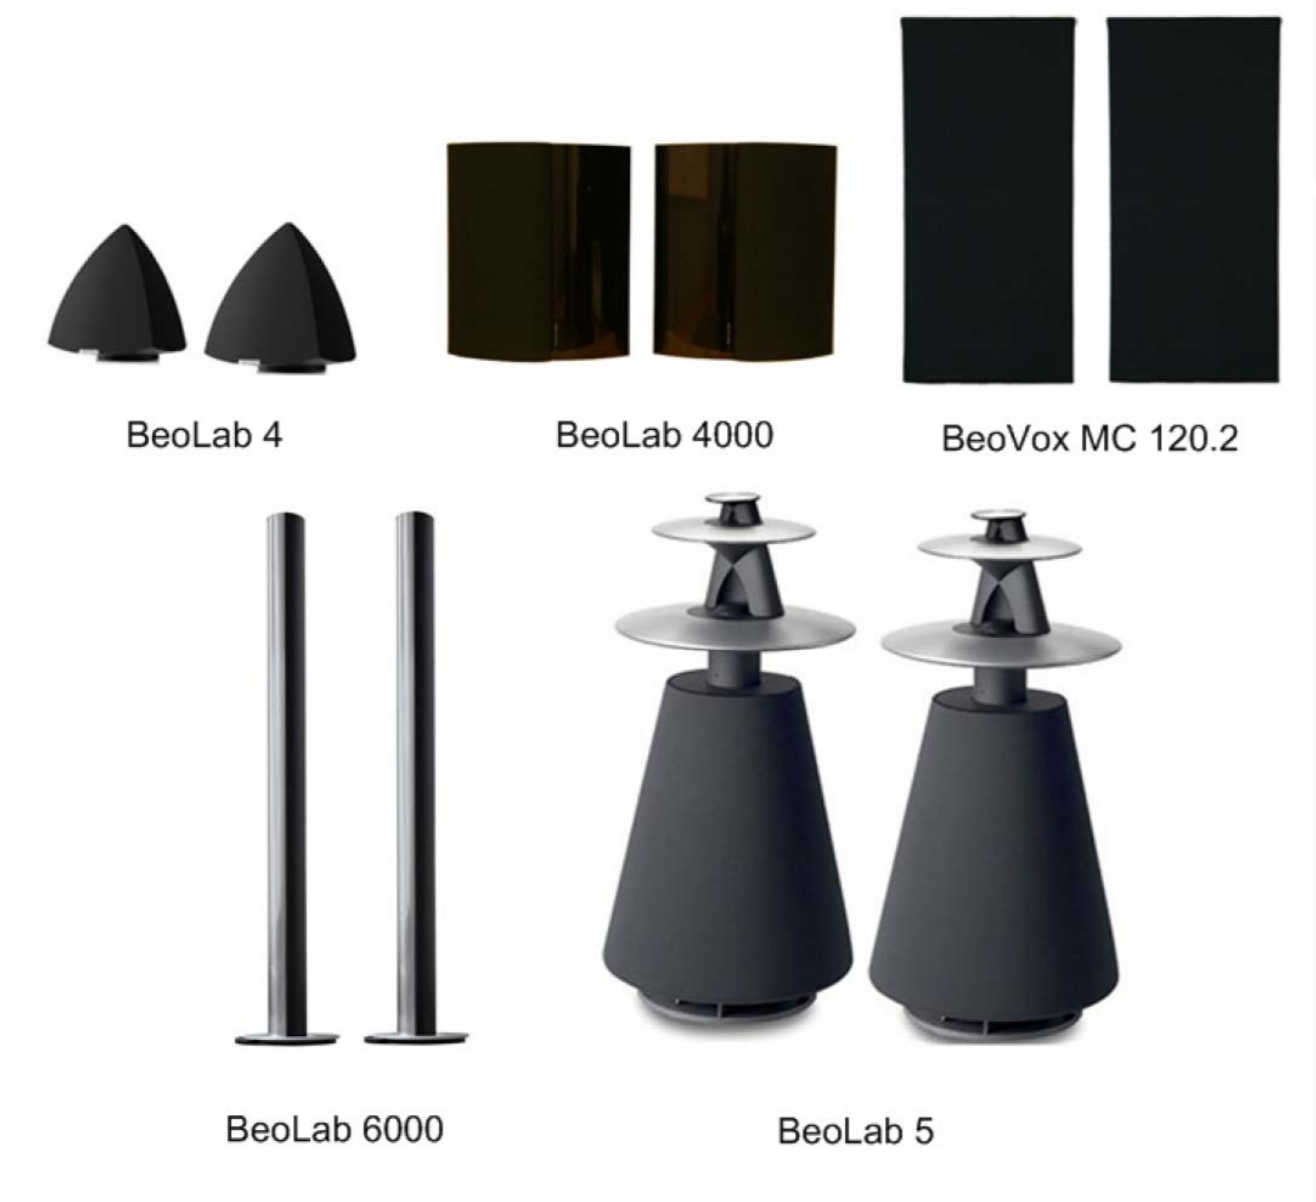
\includegraphics[scale = 0.7]{Figure/speakers.png}
\caption{Overview of the speakers used in the data set. They are all from Bang \& Olufsen in order to avoid any bias relating to specific brands.}
\label{fig:speakers}
\end{figure}
\noindent
%
The data is analyzed using the software \textit{PanelCheck}. The analysis is quite explorative, since it is still unknown what we are looking for. 

\subsection*{PanelCheck Software}
\textit{PanelCheck} is a free software which is made to be easy-to-use. It is mainly used for visualisation of sensory data which helps to gain insight in a given assessor and panel performance. The software is shown on \autoref{fig:PanelCheck}.
%
\begin{figure}[H]
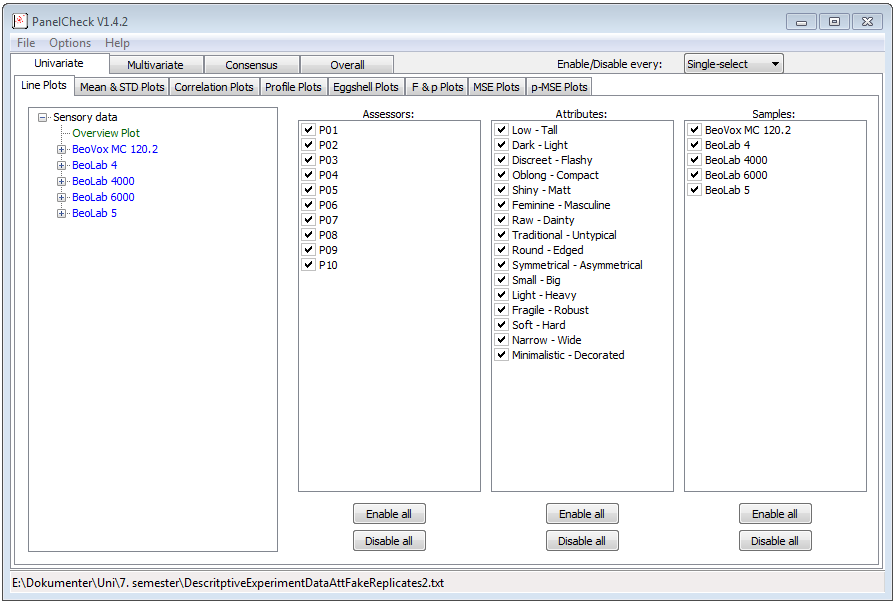
\includegraphics[width = \textwidth]{Figure/PanelCheck.png}
\caption{The start interface when \textit{PanelCheck} is started and a dataset has been imported. The 16 different attributes are shown along with the five different speakers (Samples). The ten assessors are named from P01-P10. There are four main tabs: Univariate, Multivariate, Consensus, and Overall.}
\label{fig:PanelCheck}
\end{figure}
\noindent
%
The initial interface contains an overview of the subjects (\textit{assessors}), the word-pairs (\textit{attributes}), and the different speakers (\textit{samples}). At the top it is possible to choose between different tabs: \textit{Univariate}, \textit{Multivariate}, \textit{Consensus}, or \textit{Overall}. \textit{Univariate} and \textit{Multivariate} relates to how many variables are being compared, and \textit{Consensus} relates to the underlying dimensions in the data and therefore contains PCA-related options. As the name implies, \textit{Overall} can be used to gain an overall impression of the data e.g. by showing multiple ANOVA-plots in the same calculation. Within each of the four tabs there exists varying sub-tabs which contains statistical plots relating to the chosen tab. In this example, within \textit{Univariate} it is possible to choose \textit{Line Plots}, \textit{Mean \& STD Plots}, \textit{Correlation Plots}, etc. It is also possible to exclude \textit{assessors}, \textit{attributes}, and \textit{samples}. One just have to undo the check marks in the unwanted category as shown in \autoref{fig:PanelCheck}.